\documentclass{article}
\usepackage[utf8]{inputenc}
\usepackage[T2A]{fontenc}
\usepackage[russian]{babel}
\usepackage{amsfonts}
\usepackage{amsmath}
\usepackage{amssymb}
\usepackage[left=3cm,right=3cm,top=3cm,bottom=3cm]{geometry}
\usepackage{graphicx}
\usepackage{hyperref}
\usepackage{multicol}
\usepackage{stackrel}
\usepackage{xcolor}
\usepackage{graphicx}
\usepackage{listings}
\usepackage{float}
\usepackage{listings}
\usepackage{xcolor}
\usepackage{inconsolata}
\lstset { %
	language=C++,
	backgroundcolor=\color{white!5}, % set backgroundcolor
	basicstyle=\footnotesize,% basic font setting
}
\graphicspath{ {./images/} }
\providecommand{\myceil}[1]{\left \lceil #1 \right \rceil }
\begin{document}
	\pagestyle{empty}
	\normalsize
	\newcommand{\R}{{\mathbb R}}
	\newcommand{\N}{{\mathbb N}}
	\newcommand{\lm}[2]{\displaystyle \lim_{#2 \to \infty}{#1_{#2}}}
	\newcommand{\eps}{\varepsilon}
	\begin{center}
\begin{tabular}{ |c|c|c| } 
	\hline
	Лабораторная работа №3 & М3137 & 2022 \\ 
	\hline
	Дизассемблер RISC-V & Сологуб Матвей Андреевич & \\ 
	\hline
\end{tabular}
\end{center}
	\large
\paragraph{Цель работы:}
Изучение набора команд RISC-V RV32I, RV32M. Изучение структуры ELF файла. Написание дизассемблера.
\paragraph{Инструментарий:}
Microsoft Visual C++20 / GNU C++20.
\paragraph{Описание работы:}
Распарсить ELF-файл: найти в таблице заголовков секций оффсеты необходимых секций, а именно .symtab и .text, для этого предварительно сопоставив секции из таблицы заголовков с их названиями из .shstrtab. Распарсить .symtab по найденным оффсетам, и используя метки из .symtab распарсить .text.
\paragraph{Описание системы кодирования команд RISC-V:}

\textbf{ISA} - Instruction Set Architecture - описание набора команд и регистров предоставляемых какой-либо архитектурой. \textbf{RISC-V} - Reduced Instruction Set Computer - архитектура, основанная на идеи сокращения набора команд до самых необходимых, а также разделения их на две категории: доступа к памяти(memory) и арифметические/логические(ALU). ISA RISC-V описывает интерфейс работы с данной архитектурой, а так же детали следующих наборов инструкций:
\begin{itemize}
	\item{RV32I - базовые 32-битные целочисленные инструкции}
	\item{RV32E - базовые 32-битные целочисленные инструкции}
	\item{RV64I - базовые 64-битные целочисленные инструкции}
	\item{RV128E -базовые 128-битные целочисленные инструкции}
	\item{*M - расширение, инструкции умножения и деления}
	\item{*A - расширение, атомарные инструкции}
	\item{*F - расширение, инструкции работающие с числами с плавающей точкой}
	\item{*D - расширение, инструкции работающие с числами с плавающей точкой двойной точности}
	\item{*Q - расширение, инструкции работающие с числами с плавающей точкой четверной точности}
	\item{*L - расширение, инструкции работающие с числами с десятичной плавающей точкой}
	\item{*C - расширение, сжатые инструкции}
	\item{*D - расширение, битовые операции}
	\item{*L - расширение, инструкции работающие с числами с десятичной плавающей точкой}
	\item{*J - расширение, инструкции для динамически транслируемых языков}
	\item{*P - расширение, для Packed-SIMD инструкций}
	\item{*V - расширение, векторные операции}
	\item{*Zam - расширение, дополняет атомарные инструкции}
	\item{*Ztso - расширение, Total Store Ordering}
\end{itemize}
\paragraph{Инструкции RV32I}
Набор содержащий 39 базовых целочисленных арифметических инструкций, логических инструкций, инструкций перехода, инструкций ветвления, чтения/записи данных в память и инструкций среды. Присутствуют как арифметические и логические инструкции оперирующей над двумя регистрами, и помещающие результат в третий регистр, так и инструкции которые принимают на вход регистр и константу. см. Рис1\\ 
\begin{itemize}
	\item{Инструкции чтения данных принимают адрес в виде константы и регистра, и присваивают в некоторый регистр данные находящиеся по этому адресу}
	\item{Инструкции записи наоборот присваивают в переданный адрес данные с регистра}
	\item{Инструкции перехода позволяют изменять регистр PC на некоторый оффсет, переданный в виде константы или константы+регистра. Таким образом можно нелинейно переходить на другие инструкции, создавать циклы и т.п}
	\item{Инструкции ветвления позволяют делать или не делать такие переходы в зависимости от значений на регистрах, создавая условные конструкции}
	\item{Инструкции среды могут передавать контроль операционной системе или дебагеру}
\end{itemize}
\begin{figure}[H]
		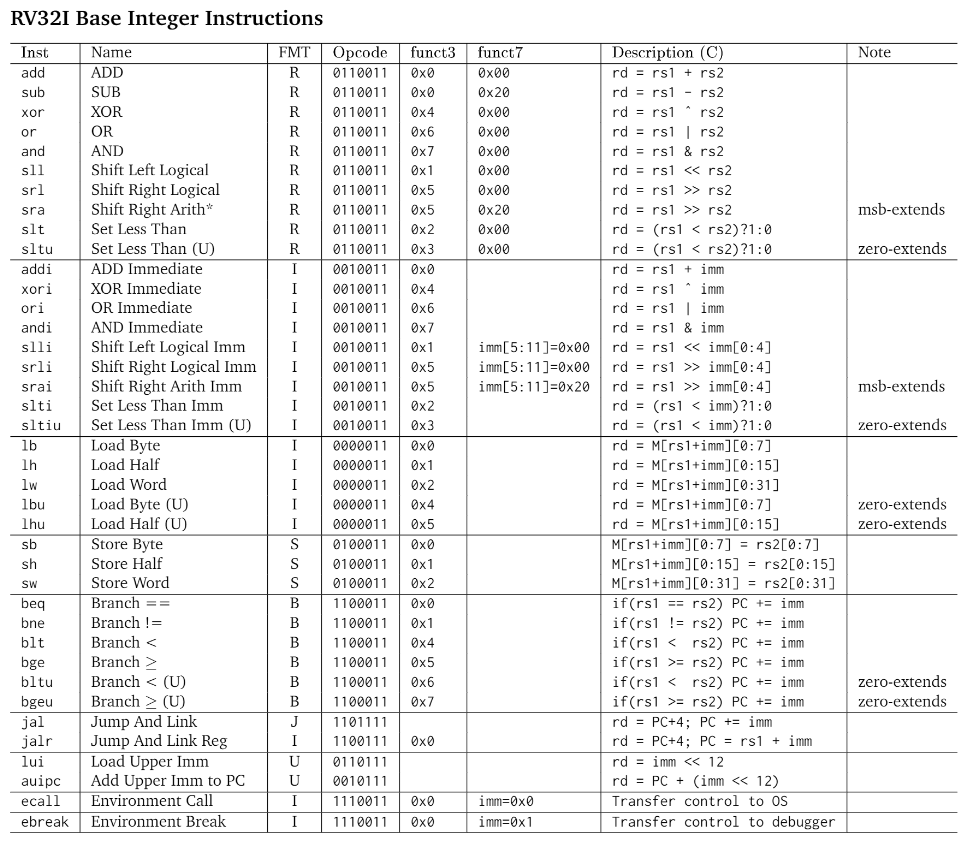
\includegraphics[width=1\textwidth]{pictures/rv32i}
		\caption{Целочисленные 32-битные инструкции}
\end{figure}
\paragraph{Инструкции RV32M}
Добавляют операции умножения, деления и взятия по остаку, в которых операндами выступают значения на двух регистрах, а результат записывается в третий регистр. см. Рис2
\begin{figure}[H]
	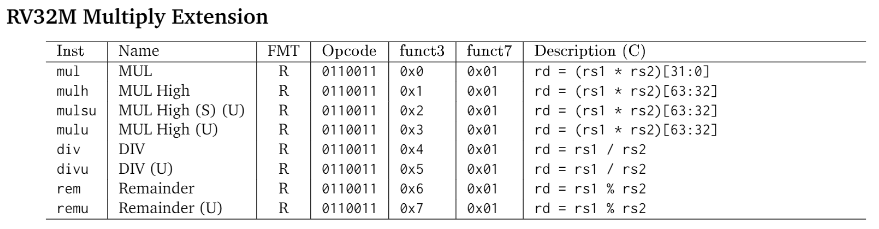
\includegraphics[width=1\textwidth]{pictures/r32m}
	\caption{Целочисленные 32-битные инструкции}
\end{figure}
\paragraph{Устройство инструкций}
Инструкции RV32I и RV32M кодируются 32 битами в формате little-endian. Существуют несколько типов инструкций, структура у разных типов различается. Во всех инструкциях младшие 7 бит обозначают opcode, который однозначно задаёт расположение следующих полей. 
\\
\begin{figure}[H]
	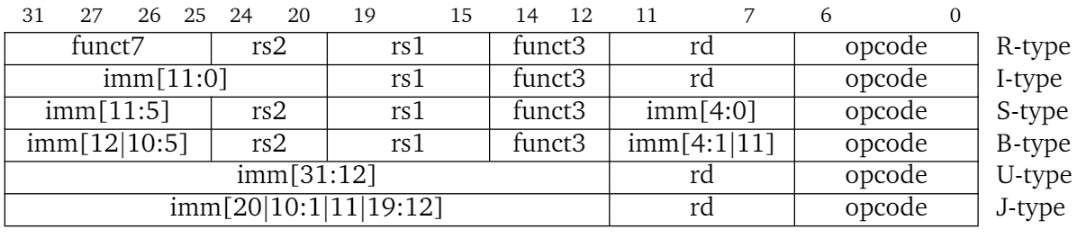
\includegraphics[width=1\textwidth]{pictures/instructionTypes}
	\caption{Типы инструкций}
\end{figure}
Поля \textbf{rs1}, \textbf{rs2} и \textbf{rd} содержат коды регистров над которыми производится операция. Поле \textbf{imm} содержит некоторую константу в форме дополнения до двух, в зависимости от инструкции она может быть интерпретирована по разному. Поля \textbf{funct3} и \textbf{funct7} содержат информацию для дифференциации инструкций внутри одного класса. Значение в поле \textbf{imm} стоит сдвигать на 1 бит влево, так как там хранится число кратное двум и младший бит опущен для экономии места. Так же оно может быть разбито на несколько частей другими полями. см. Рис3\\
Так же существует 32 целочисленных регистра и 32 регистра для чисел с плавающей точкой и дополнительный регистр \textbf{pc} указывающий на текущую инструкцию (именно он используется в прыжках и инструкциях ветвления) см. Рис 4
\begin{figure}[H]
	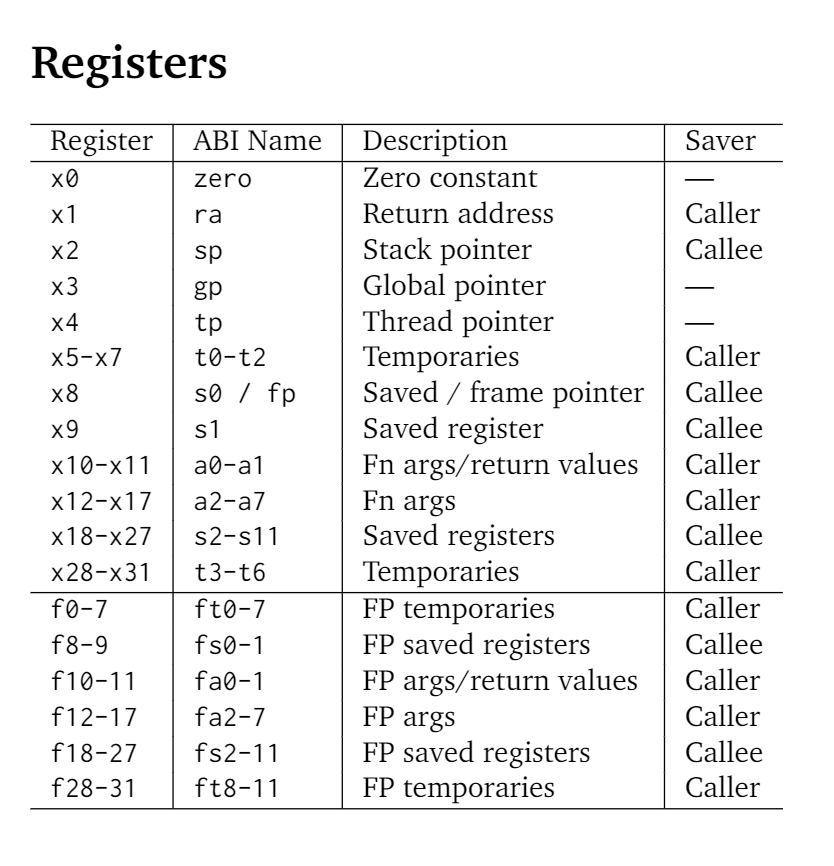
\includegraphics[width=1\textwidth]{pictures/registers}
	\caption{Регистры}
\end{figure}
\section*{Структура ELF-файла}
\textbf{ELF} - Executable and Linkable Format, формат исполняемых и компонуемых файлов. Содержит в себе информацию о программе и исполняемый код. Бывает как ELF64 так и ELF32 отличающиеся размером некоторых разделов, но так как мы рассматриваем 32-битный вариант, речь будет идти лишь о нём.
\paragraph{Заголовок файла}
Занимает первые 52 байта в файле. Первые 4 байта содержат сигнатуру ELF-файла, если они отличаются от $0x464c457f$, это не ELF-файл! Далее идут различные данные о файле, такие как его тип (исполняемый/объектный и т.п), архитектура для которой он предназначен, версия ELF и оффсеты различных секций файла, которые как раз нам и нужны. Отсюда мы возьмём: Адрес точки входа в программу (от него будут исчисляться адреса инструкций), оффсет на таблицу заголовков секций (в ней и содержатся данные о секциях .text и .symtab), число заголовков секций и номер заголовка, содержащего информацию о секции описывающей таблицу названия секций.
\paragraph{Таблица заголовков секций}
Зная её местоположение, размер одного заголовка(32 байта) и количество заголовков, мы можем итерироваться по ним и рассматривать каждый по отдельности. Каждый заголовок содержит в себе: смещение строки, содержащей название данной секции (необходимо чтобы узнать название секции из таблицы имён секций), тип заголовка, оффсет самой секции (начиная с него мы и будем считывать данные), размер секции, размер каждой записи. Теперь сопоставив каждой секции её название из секции с названиями (читаем по данному нам оффсету обычную си-строку), мы знаем оффсеты на секции .text и .symtab.
\paragraph{.symtab}
\textbf{Symbol Table} - таблица символов, длина одного вхождения - 16 байт, состоит из:
\begin{itemize}
	\item{Оффсет имени - 4 байта}
	\item{Значение - 4 байта}
	\item{Размер - 4 байт}
	\item{Информация - 1 байт}
	\item{Другое - 1 байт}
	\item{Индекс - 2 байта}
\end{itemize}
Имена берём также, только уже из секции .strtab. По оффсету 96 бит от начала записи берём 4 бита - это тип символа. По оффсету 100, 4 бита - биндинг символа. По оффсету 104 берём 8 бит - видимость символа. 
\section*{Описание работы программы}
\paragraph{Общая структура}
Компиляция: g++ disasm.cpp -std=c++2a -o rv3.exe\\
Всего в проекте два файла: disasm.cpp и constants.h . Файл disasm.cpp содержит функцию main, несколько структур и методов. constants.h содержит все константы, оффсеты, сопоставления значений именам.\\
\textbf{Метод read}, считываем size бит по адресу offset от начала файла (в битах)
\begin{figure}[H]
	\begin{lstlisting}
uint32_t read(int offset, int size) {
	if(!(0 <= size || size <= 32)){
		std::cout << "Wrong size given: " + size << '\n';
		return 0;
	}
	uint32_t output = 0;
	for (int i = offset; i < offset + size; ++i){
		int ind = i / 8;
		int lPos = i % 8;
		output |= ((1 & input[ind] >> lPos) << i - offset);
	}
	return output;
}
	\end{lstlisting}
\caption{Метод read()}
\end{figure}
\textbf{Метод toSigned()}, превращает беззнаковое число в форму дополнение до двух
\begin{figure}[H]
	\begin{lstlisting}
int toSigned(int n, int size){
	if ((n & (1 << (size - 1)))){
		return(n | ~((1 << size) - 1));
	}
	else{
		return(n);
	}
}
	\end{lstlisting}
	\caption{Метод toSigned()}
\end{figure}
\paragraph{Выполнение main}
Считываем аргументы, если их кол-во меньше двух - выводим ошибку и выходим. Проверяем наличие самого файла, если нет - выводим ошибку. Далее пытаемся прочесть файл в массив байт - input. Закрываем поток, проверяем сигнатуру, и архитектуру. Если всё совпало начинаем парсить нужные данные из первых 52 байт, такие как оффсет на таблицу секций и т.п (уже расписал в отделе про ELF).
\begin{figure}[H]
	\begin{lstlisting}
uint32_t sectionHeadersTableOffset = read(e_shoff_off * 8, 32);
uint16_t sectionSize = read(e_shentsize_off * 8, 16);
uint16_t sectionCount = read(e_shnum_off * 8, 16);
uint16_t sectionOfNamesIndex = read(e_shstrndx_off * 8, 16);
	\end{lstlisting}
	\caption{Парсим заголовок}
\end{figure}
Далее, я сделал лямбду которая будет парсить каждую секцию (почему не метод? да по приколу):
\begin{figure}[H]
	\begin{lstlisting}
auto parseSection = [&](uint16_t i, uint32_t& Offset, uint32_t& NameOffset, uint32_t& size) {
int sechOff = sectionHeadersTableOffset + i * sectionSize;
NameOffset = read(sechOff * 8, 32);
Offset = read(sechOff * 8 + 16 * 8, 32);
size = read(sechOff * 8 + 20 * 8, 32);
};
	\end{lstlisting}
	\caption{Парсим секцию}
\end{figure}
Для хранения секций сделал структурку:
\begin{figure}[H]
	\begin{lstlisting}
struct section {
	uint32_t offset;
	uint32_t size;
};
	\end{lstlisting}
	\caption{Секция}
\end{figure}
Теперь с помощью лямбды парсим секцию с именами секций, чтобы когда мы будем парсить все секции у нас уже были их имена. Добавляем их в заранее созданную мапу по именам:
\begin{figure}[H]
	\begin{lstlisting}
for (int i = 0; i < sectionCount; ++i) {
	uint32_t sectionOffset = 0, sectionNameOffset = 0, sectionSize = 0;
	parseSection(i, sectionOffset, sectionNameOffset, sectionSize);
	std::string name = "";
	int k = namesTableOffset + sectionNameOffset;
	while (read(k * 8, 8) != '\0') {
		name += (char)read(k * 8, 8);
		++k;
	}
	sections[name] = section{sectionOffset, sectionSize};
}
	\end{lstlisting}
	\caption{Парсим много секций}
\end{figure}
Теперь когда у нас есть мапа Имя $\rightarrow$ Секция, мы можем взять из неё нужные секции, а именно .symtab и .text и заняться их парсингом.
Заведём структурку и для символов:
\begin{figure}[H]
	\begin{lstlisting}
struct symbol{
	uint32_t num;
	uint32_t value;
	uint32_t size;
	std::string type;
	std::string bind;
	std::string vis;
	std::string ndx;
	std::string name;
};
	\end{lstlisting}
	\caption{Символ}
\end{figure}
\begin{figure}[H]
	\begin{lstlisting}
int symtabOff = sections[".symtab"].offset;
int symSize = sections[".symtab"].size;
int strtabOff = sections[".strtab"].offset;
std::vector<symbol> symbols(symSize / 16);
for (int symOff = symtabOff, num = 0; symOff < symtabOff + symSize; symOff += 16, ++num){
	uint32_t st_name = read(symOff * 8, 32);
	uint32_t st_value = read((symOff + 4) * 8, 32);
	uint32_t st_size = read((symOff + 8) * 8, 32);
	uint16_t st_shndx = read((symOff + 14) * 8, 16);
	std::string ndx = ndx_state.contains(st_shndx) ? ndx_state[st_shndx] : std::to_string(st_shndx);
	std::string type = st_type[read((symOff + 12) * 8, 4)];
	std::string bind = st_binding[read((symOff + 12) * 8 + 4, 4)];
	std::string visibility = st_visibility[read((symOff + 13) * 8, 8)];
	int k = strtabOff + st_name;
	std::string name;
	while (read(k * 8, 8) != '\0'){
		name += (char)read(k * 8, 8);
		++k;
	}
	symbols[num] = {(uint32_t)num, st_value, st_size, type, bind, visibility, ndx, name};
}
	\end{lstlisting}
	\caption{Парсим .symtab}
\end{figure}
	Самое время приступать к парсу .text, но перед этим заведём две мапы маркеров вида Адрес $\rightarrow$ Имя и счётчик, и положим в мапу bigMarkers все символы из .symtab'а, позже нам это пригодится. Парсим инструкции: Сначала считываем opcode, а потом в зависимости от типа инструкции (R,I и т.п) парсим то что есть из funct3, funct7, rs1, rs2, rd, imm. Далее заносим инструкцию в мапу следующего вида: Адрес $\rightarrow$ Инструкция. В целом все они парсятся похоже, если какого-то элемента нет, (отсутствует rs2 или imm например), то он просто зануляется. Но на B инструкциях и на jal происходит кое-что интересное: так как они могут совершать переходы на оффсет imm, мы должны поставить им маркер. Смотрим в bigMarkers[addr+imm], если такой маркер есть, то присваиваем его в smallMarkers[addr], если нет - то ставим $L_{markersCount}$ и присваиваем его в bigMarkers[addr+imm] и smallMarkers[addr], увеличивая markersCount. Таким образом в конце в bigMarkers у нас окажутся все маркеры которые должны занимать строку, а в smallMarkers все маркеры которые должны выводиться в конце инструкции.
\begin{figure}[H]
	\begin{lstlisting}
uint8_t funct3 = read(off + 12, 3);
uint8_t rs1 = read(off + 15, 5);
uint8_t rs2 = read(off + 20, 5);
int imm = 0;
imm |= (read(off + 31, 1) << 12);
for (int i = 10; i >= 5; i--){
	imm |= (read(off + 20 + i, 1) << i);
}
for (int i = 4; i >= 1; i--){
	imm |= (read(off + 7 + i, 1) << i);
}
imm |= (read(off + 7, 1) << 11);
std::string name = B_instruction[{funct3, 0}];
imm = toSigned(imm, 13);
if (bigMarkers.contains(addr + imm)){
	smallMarkers[addr] = bigMarkers[addr + imm];
}
else{
	std::string marker = "<L" + std::to_string(markersCount) + ">";
	smallMarkers[addr] = marker;
	bigMarkers[addr + imm] = marker;
	++markersCount;
}
instructions[addr] = {name, raw, "", reg[rs1],reg[rs2], imm, opCode[op]};
	\end{lstlisting}
	\caption{Пример парса B инструкций}
\end{figure}
Теперь когда у нас есть всё необходимое, открываем поток на запись, и идя по мапе с инструкциями выводим каждую в нужном для неё формате, вставляя там где надо маркеры. Также в нужном формате выводим массив символов из .symtab. Закрываем поток на запись.
\section*{Результат работы на тестовом файле:}
\begin{lstlisting}
00010074   <main>:
10074:	ff010113	   addi	sp, sp -16
10078:	00112623	     sw	ra, 12(sp)
1007c:	030000ef	    jal	ra, 0x100ac <mmul>
10080:	00c12083	     lw	ra, 12(sp)
10084:	00000513	   addi	a0, zero 0
10088:	01010113	   addi	sp, sp 16
1008c:	00008067	   jalr	zero, 0(ra)
10090:	00000013	   addi	zero, zero 0
10094:	00100137	    lui	sp, 256
10098:	fddff0ef	    jal	ra, 0x10074 <main>
1009c:	00050593	   addi	a1, a0 0
100a0:	00a00893	   addi	a7, zero 10
100a4:	00000000		unknown_instruction
100a8:	00000073	  ecall
000100ac   <mmul>:
100ac:	00011f37	    lui	t5, 17
100b0:	124f0513	   addi	a0, t5 292
100b4:	65450513	   addi	a0, a0 1620
100b8:	124f0f13	   addi	t5, t5 292
100bc:	e4018293	   addi	t0, gp -448
100c0:	fd018f93	   addi	t6, gp -48
100c4:	02800e93	   addi	t4, zero 40
000100c8   <L2>:
100c8:	fec50e13	   addi	t3, a0 -20
100cc:	000f0313	   addi	t1, t5 0
100d0:	000f8893	   addi	a7, t6 0
100d4:	00000813	   addi	a6, zero 0
000100d8   <L1>:
100d8:	00088693	   addi	a3, a7 0
100dc:	000e0793	   addi	a5, t3 0
100e0:	00000613	   addi	a2, zero 0
000100e4   <L0>:
100e4:	00078703	     lb	a4, 0(a5)
100e8:	00069583	     lh	a1, 0(a3)
100ec:	00178793	   addi	a5, a5 1
100f0:	02868693	   addi	a3, a3 40
100f4:	02b70733	    mul	a4, a4, a1
100f8:	00e60633	    add	a2, a2, a4
100fc:	fea794e3	    bne	a5, a0 0x100e4 <L0>
10100:	00c32023	     sw	a2, 0(t1)
10104:	00280813	   addi	a6, a6 2
10108:	00430313	   addi	t1, t1 4
1010c:	00288893	   addi	a7, a7 2
10110:	fdd814e3	    bne	a6, t4 0x100d8 <L1>
10114:	050f0f13	   addi	t5, t5 80
10118:	01478513	   addi	a0, a5 20
1011c:	fa5f16e3	    bne	t5, t0 0x100c8 <L2>
10120:	00008067	   jalr	zero, 0(ra)

.symtab
Symbol Value          	Size Type 	Bind 	Vis   	Index Name
[   0] 0x0                   0 NOTYPE   LOCAL    DEFAULT   UNDEF 
[   1] 0x10074               0 SECTION  LOCAL    DEFAULT       1 
[   2] 0x11124               0 SECTION  LOCAL    DEFAULT       2 
[   3] 0x0                   0 SECTION  LOCAL    DEFAULT       3 
[   4] 0x0                   0 SECTION  LOCAL    DEFAULT       4 
[   5] 0x0                   0 FILE     LOCAL    DEFAULT     ABS test.c
[   6] 0x11924               0 NOTYPE   GLOBAL   DEFAULT     ABS __global_pointer$
[   7] 0x118F4             800 OBJECT   GLOBAL   DEFAULT       2 b
[   8] 0x11124               0 NOTYPE   GLOBAL   DEFAULT       1 __SDATA_BEGIN__
[   9] 0x100AC             120 FUNC     GLOBAL   DEFAULT       1 mmul
[  10] 0x0                   0 NOTYPE   GLOBAL   DEFAULT   UNDEF _start
[  11] 0x11124            1600 OBJECT   GLOBAL   DEFAULT       2 c
[  12] 0x11C14               0 NOTYPE   GLOBAL   DEFAULT       2 __BSS_END__
[  13] 0x11124               0 NOTYPE   GLOBAL   DEFAULT       2 __bss_start
[  14] 0x10074              28 FUNC     GLOBAL   DEFAULT       1 main
[  15] 0x11124               0 NOTYPE   GLOBAL   DEFAULT       1 __DATA_BEGIN__
[  16] 0x11124               0 NOTYPE   GLOBAL   DEFAULT       1 _edata
[  17] 0x11C14               0 NOTYPE   GLOBAL   DEFAULT       2 _end
[  18] 0x11764             400 OBJECT   GLOBAL   DEFAULT       2 a
\end{lstlisting}
\section*{Список источников}
\url{https://ru.wikipedia.org/wiki/Executable_and_Linkable_Format}\\
\url{https://docs.oracle.com/cd/E19683-01/817-3677/chapter6-94076/index.html}\\
\url{https://github.com/jameslzhu/riscv-card/blob/master/riscv-card.pdf}\\
\url{https://refspecs.linuxbase.org/elf/gabi4+/ch4.symtab.html}
\section*{Листинг кода}
	\begin{lstlisting}
diasm.cpp

#include <iostream>
#include <fstream>
#include <string>
#include <filesystem>
#include <cassert>
#include "constants.h"


inline uint32_t getFileSize(const std::string& filename) {
	std::filesystem::path p(filename);
	return std::filesystem::file_size(p);
}

inline bool fileExists(const std::string& filename) {
	std::filesystem::path p(filename);
	return std::filesystem::exists(p);
}

std::vector<uint8_t> input;

uint32_t read(int offset, int size) {
	assert(0 <= size || size <= 32);
	uint32_t output = 0;
	for (int i = offset; i < offset + size; ++i){
		int ind = i / 8;
		int lPos = i % 8;
		output |= ((1 & input[ind] >> lPos) << i - offset);
	}
	return output;
}

struct section {
	uint32_t offset;
	uint32_t size;
};

struct symbol{
	uint32_t num;
	uint32_t value;
	uint32_t size;
	std::string type;
	std::string bind;
	std::string vis;
	std::string ndx;
	std::string name;
};

struct instruction{
	std::string name;
	uint32_t raw;
	std::string rd;
	std::string rs1;
	std::string rs2;
	int imm;
	std::string type;
};

int toSigned(int n, int size){
	if ((n & (1 << (size - 1)))){
		return(n | ~((1 << size) - 1));
	}
	else{
		return(n);
	}
}

int main(int argc, char* argv[]) {
	std::vector<std::string> args;
	for (int i = 0; i < argc; i++) {
		args.push_back(argv[i]);
	}
	if (args.size() < 3){
		std::cout << "Expected 2 arguments, but " + std::to_string(args.size() - 1) + " provided\n";
		return 0;
	}
	std::string inputName = args[1];
	std::string outputName = args[2];
	if (!fileExists(inputName)) {
		std::cout << "Error! File doesn't exist\n";
		return 0;
	}
	int inputSize = getFileSize(inputName);
	if (inputSize < 52 + 32) {
		std::cout << "File is too small to be ELF\n";
		return 0;
	}
	std::ifstream inputStream(inputName, std::ios_base::binary);
	input = std::vector<uint8_t>(inputSize);
	try{
		inputStream.read(reinterpret_cast<char*>(&input[0]), inputSize);
	}
	catch (...){
		std::cout << "Can't read this file!";
		inputStream.close();
		return 0;
	}
	inputStream.close();
	
	uint32_t fileSignature = read(0, 32);
	if (fileSignature != elf_signature) {
		std::cout << "It's not an ELF file!\n";
		return 0;
	}
	uint16_t fileArchitecture = read(e_machine_off * 8, 16);
	if (fileArchitecture != riscv_signature) {
		std::cout << "Architecture is not RISC-V, can't handle it...\n";
		return 0;
	}
	uint32_t sectionHeadersTableOffset = read(e_shoff_off * 8, 32);
	uint16_t sectionSize = read(e_shentsize_off * 8, 16);
	uint16_t sectionCount = read(e_shnum_off * 8, 16);
	uint16_t sectionOfNamesIndex = read(e_shstrndx_off * 8, 16);
	std::unordered_map<std::string, section> sections;
	auto parseSection = [&](uint16_t i, uint32_t& Offset, uint32_t& NameOffset, uint32_t& size) {
		int sechOff = sectionHeadersTableOffset + i * sectionSize;
		NameOffset = read(sechOff * 8, 32);
		Offset = read(sechOff * 8 + 16 * 8, 32);
		size = read(sechOff * 8 + 20 * 8, 32);
	};
	uint32_t namesTableOffset = -1, namesTableNameOffsetxD = -1, namesTableSize;
	parseSection(sectionOfNamesIndex, namesTableOffset, namesTableNameOffsetxD, namesTableSize);
	for (int i = 0; i < sectionCount; ++i) {
		uint32_t sectionOffset = 0, sectionNameOffset = 0, sectionSize = 0;
		parseSection(i, sectionOffset, sectionNameOffset, sectionSize);
		std::string name = "";
		int k = namesTableOffset + sectionNameOffset;
		while (read(k * 8, 8) != '\0') {
			name += (char)read(k * 8, 8);
			++k;
		}
		sections[name] = section{sectionOffset, sectionSize};
	}
	int symtabOff = sections[".symtab"].offset;
	int symSize = sections[".symtab"].size;
	int strtabOff = sections[".strtab"].offset;
	std::vector<symbol> symbols(symSize / 16);
	for (int symOff = symtabOff, num = 0; symOff < symtabOff + symSize; symOff += 16, ++num){
		uint32_t st_name = read(symOff * 8, 32);
		uint32_t st_value = read((symOff + 4) * 8, 32);
		uint32_t st_size = read((symOff + 8) * 8, 32);
		uint16_t st_shndx = read((symOff + 14) * 8, 16);
		std::string ndx = ndx_state.contains(st_shndx) ? ndx_state[st_shndx] : std::to_string(st_shndx);
		std::string type = st_type[read((symOff + 12) * 8, 4)];
		std::string bind = st_binding[read((symOff + 12) * 8 + 4, 4)];
		std::string visibility = st_visibility[read((symOff + 13) * 8, 8)];
		int k = strtabOff + st_name;
		std::string name;
		while (read(k * 8, 8) != '\0'){
			name += (char)read(k * 8, 8);
			++k;
		}
		symbols[num] = {(uint32_t)num, st_value, st_size, type, bind, visibility, ndx, name};
	}
	std::unordered_map<uint32_t, std::string> bigMarkers, smallMarkers;
	int markersCount = 0;
	for (const auto& v : symbols){
		bigMarkers[v.value] = "<" + v.name + ">";
	}
	int textOff = sections[".text"].offset;
	int textSize = sections[".text"].size;
	uint32_t entryPoint = read(e_entry_off * 8, 32);
	std::map<uint32_t, instruction> instructions;
	for (int off = textOff * 8, addr = entryPoint; off < (textOff + textSize) * 8; off += 32, addr += 4){
		uint8_t op = read(off, 7);
		uint32_t raw = read(off, 32);
		if (opCode[op] == "R"){
			uint8_t rd = read(off + 7, 5);
			uint8_t funct3 = read(off + 12, 3);
			uint8_t rs1 = read(off + 15, 5);
			uint8_t rs2 = read(off + 20, 5);
			uint8_t funct7 = read(off + 25, 7);
			std::string name = R_instruction[{funct3, funct7}];
			instructions[addr] = {name,raw,reg[rd], reg[rs1], reg[rs2], 0, opCode[op]};
		}
		else if (opCode[op][0] == 'I'){
			uint8_t rd = read(off + 7, 5);
			uint8_t funct3 = read(off + 12, 3);
			uint8_t funct7 = 0;
			uint8_t rs1 = read(off + 15, 5);
			int imm = read(off + 20, 12);
			if (opCode[op] == "I" && funct3 == 0x5){
				funct7 = read(off + 25, 7);
			}
			if (opCode[op] == "Ie"){
				funct7 = read(off + 20, 12);
			}
			std::string name;
			if (opCode[op] == "I"){
				name = I_instruction[{funct3, funct7}];
			}
			else if (opCode[op] == "Il"){
				name = Il_instruction[{funct3, 0}];
			}
			else if (opCode[op] == "Ij"){
				name = Ij_instruction[{0, 0}];
			}
			else if (opCode[op] == "Ie"){
				name = Ie_instruction[{0, funct7}];
			}
			imm = toSigned(imm, 12);
			instructions[addr] = {name, raw, reg[rd], reg[rs1],"", imm, opCode[op]};
		}
		else if (opCode[op] == "S"){
			int imm = 0;
			for (int i = 11; i >= 5; --i){
				imm |= (read(off + 20 + i, 1) << i);
			}
			for (int i = 4; i >= 0; --i){
				imm |= (read(off + 7 + i, 1) << i);
			}
			uint8_t funct3 = read(off + 12, 3);
			uint8_t rs1 = read(off + 15, 5);
			uint8_t rs2 = read(off + 20, 5);
			std::string name = S_instruction[{funct3, 0}];
			imm = toSigned(imm, 12);
			instructions[addr] = {name, raw, "", reg[rs1],reg[rs2], imm, opCode[op]};
		}
		else if (opCode[op] == "B"){
			uint8_t funct3 = read(off + 12, 3);
			uint8_t rs1 = read(off + 15, 5);
			uint8_t rs2 = read(off + 20, 5);
			int imm = 0;
			imm |= (read(off + 31, 1) << 12);
			for (int i = 10; i >= 5; i--){
				imm |= (read(off + 20 + i, 1) << i);
			}
			for (int i = 4; i >= 1; i--){
				imm |= (read(off + 7 + i, 1) << i);
			}
			imm |= (read(off + 7, 1) << 11);
			std::string name = B_instruction[{funct3, 0}];
			imm = toSigned(imm, 13);
			if (bigMarkers.contains(addr + imm)){
				smallMarkers[addr] = bigMarkers[addr + imm];
			}
			else{
				std::string marker = "<L" + std::to_string(markersCount) + ">";
				smallMarkers[addr] = marker;
				bigMarkers[addr + imm] = marker;
				++markersCount;
			}
			instructions[addr] = {name, raw, "", reg[rs1],reg[rs2], imm, opCode[op]};
		}
		else if (opCode[op][0] == 'U'){
			int imm = read(off + 12, 20);
			uint8_t rd = read(off + 7, 5);
			std::string name;
			if (opCode[op] == "Ul"){
				name = Ul_instruction[{0, 0}];
			}
			else{
				name = Ua_instruction[{0, 0}];
			}
			imm = toSigned(imm, 21);
			instructions[addr] = {name, raw, reg[rd], "", "", imm, opCode[op]};
		}
		else if (opCode[op] == "J"){
			int imm = 0;
			imm |= (read(off + 31, 1) << 20);
			for (int i = 10; i >= 1; i--){
				imm |= (read(off + 20 + i, 1) << i);
			}
			imm |= (read(off + 20, 1) << 11);
			for (int i = 19; i >= 12; i--){
				imm |= (read(off + i, 1) << i);
			}
			uint8_t rd = read(off + 7, 5);
			std::string name = J_instruction[{0, 0}];
			imm = toSigned(imm, 21);
			if (name == "jal"){
				if (bigMarkers.contains(addr + imm)){
					smallMarkers[addr] = bigMarkers[addr + imm];
				}
				else{
					std::string marker = "<L" + std::to_string(markersCount) + ">";
					smallMarkers[addr] = marker;
					bigMarkers[addr + imm] = marker;
					++markersCount;
				}
			}
			imm = toSigned(imm, 21);
			instructions[addr] = {name, raw, reg[rd], "", "", imm, opCode[op]};
		}
		else{
			instructions[addr] = {"",0,"","","",0, "unknown_instruction"};
		}
	}
	FILE* file = 0;
	int errCode = fopen_s(&file, outputName.c_str(), "w");
	if (errCode){
		std::cout << "Can't open file " + outputName + " for write, error code: " + std::to_string(errCode) << '\n';
	}
	for (auto& [addr, inst] : instructions){
		if (bigMarkers.contains(addr)){
			fprintf(file, "%08x   %s:\n", addr, bigMarkers[addr].c_str());
		}
		if (inst.type == "R"){
			fprintf(file, "   %05x:\t%08x\t%7s\t%s, %s, %s\n",
			addr, inst.raw, inst.name.c_str(), inst.rd.c_str(), inst.rs1.c_str(), inst.rs2.c_str());
		}
		else if (inst.type[0] == 'I'){
			if (inst.type == "Il" || inst.type == "Ij"){
				fprintf(file, "   %05x:\t%08x\t%7s\t%s, %d(%s)\n",
				addr, inst.raw, inst.name.c_str(), inst.rd.c_str(), inst.imm, inst.rs1.c_str());
			}
			else if (inst.type == "Ie"){
				fprintf(file, "   %05x:\t%08x\t%7s\n", addr, inst.raw, inst.name.c_str());
			}
			else{
				fprintf(file, "   %05x:\t%08x\t%7s\t%s, %s %d\n",
				addr, inst.raw, inst.name.c_str(), inst.rd.c_str(), inst.rs1.c_str(), inst.imm);
			}
		}
		else if (inst.type == "S"){
			fprintf(file, "   %05x:\t%08x\t%7s\t%s, %d(%s)\n",
			addr, inst.raw, inst.name.c_str(), inst.rs2.c_str(), inst.imm, inst.rs1.c_str());
		}
		else if (inst.type == "B"){
			fprintf(file, "   %05x:\t%08x\t%7s\t%s, %s 0x%x %s\n",
			addr, inst.raw, inst.name.c_str(), inst.rs1.c_str(), inst.rs2.c_str(), addr + inst.imm, smallMarkers[addr].c_str());
		}
		else if (inst.type == "J"){
			fprintf(file, "   %05x:\t%08x\t%7s\t%s, 0x%x %s\n",
			addr, inst.raw, inst.name.c_str(), inst.rd.c_str(), addr + inst.imm, smallMarkers[addr].c_str());
		}
		else if (inst.type[0] == 'U'){
			fprintf(file, "   %05x:\t%08x\t%7s\t%s, %d\n",
			addr, inst.raw, inst.name.c_str(), inst.rd.c_str(), inst.imm);
		}
		else if (inst.type == "unknown_instruction"){
			fprintf(file, "   %05x:\t%08x\t\t%7s\n",
			addr, inst.raw, inst.type.c_str());
		}
	}
	fprintf(file, "\n.symtab\nSymbol Value          	Size Type 	Bind 	Vis   	Index Name\n");
	for (const auto& v : symbols){
		fprintf(file, "[%4i] 0x%-15X %5i %-8s %-8s %-8s %6s %s\n", v.num, v.value, v.size, v.type.c_str(), v.bind.c_str(), v.vis.c_str(), v.ndx.c_str(), v.name.c_str());
	}
	fclose(file);
}

\end{lstlisting}
\begin{lstlisting}
constants.h
#include <algorithm>
#include <unordered_map>
#include <map>
constexpr int elf_signature = 0x464c457f;
constexpr int riscv_signature = 0xf3;

constexpr int e_machine_off = 18;
constexpr int e_shoff_off = 32;
constexpr int e_shentsize_off = 46;
constexpr int e_shnum_off = 48;
constexpr int e_shstrndx_off = 50;
constexpr int e_entry_off = 24;

inline std::unordered_map<uint8_t, std::string> opCode = {
	{0b0110011, "R"},
	{0b0010011, "I"},
	{0b0000011, "Il"},
	{0b0100011, "S"},
	{0b1100011, "B"},
	{0b1101111, "J"},
	{0b1100111, "Ij"},
	{0b0110111, "Ul"},
	{0b0010111, "Ua"},
	{0b1110011, "Ie"}
};
inline std::map<std::pair<uint16_t, uint16_t>, std::string> R_instruction = {
	{{0,0}, "add"},
	{{0, 0x20}, "sub"},
	{{0x4, 0}, "xor"},
	{{0x6, 0}, "or"},
	{{0x7, 0}, "and"},
	{{0x1, 0}, "sli"},
	{{0x5, 0}, "srl"},
	{{0x5, 0x20}, "sra"},
	{{0x2, 0}, "slt"},
	{{0x3, 0}, "sltu"},
	{{0x0, 0x1}, "mul"},
	{{0x1, 0x1}, "mulh"},
	{{0x2, 0x1}, "mulsu"},
	{{0x3, 0x1}, "mulu"},
	{{0x4, 0x1}, "div"},
	{{0x5, 0x1}, "divu"},
	{{0x6, 0x1}, "rem"},
	{{0x7, 0x1}, "remu"}
};
inline std::map<std::pair<uint16_t, uint16_t>, std::string> I_instruction = {
	{{0,0}, "addi"},
	{{0x4, 0}, "xori"},
	{{0x6, 0}, "ori"},
	{{0x7, 0}, "0"},
	{{0x1, 0}, "slli"},
	{{0x5, 0}, "srli"},
	{{0x5, 0x20}, "srai"},
	{{0x2, 0}, "slti"},
	{{0x3, 0}, "sltiu"}
};
inline std::map<std::pair<uint16_t, uint16_t>, std::string> Il_instruction = {
	{{0,0}, "lb"},
	{{0x1,0}, "lh"},
	{{0x2,0}, "lw"},
	{{0x4,0}, "lbu"},
	{{0x5,0}, "lhu"}
};
inline std::map<std::pair<uint16_t, uint16_t>, std::string> Ij_instruction = {
	{{0,0}, "jalr"},
};
inline std::map<std::pair<uint16_t, uint16_t>, std::string> Ie_instruction = {
	{{0,0}, "ecall"},
	{{0, 0x1}, "ebreak"}
};
inline std::map<std::pair<uint16_t, uint16_t>, std::string> S_instruction = {
	{{0,0}, "sb"},
	{{0x1,0}, "sh"},
	{{0x2,0}, "sw"},
};
inline std::map<std::pair<uint16_t, uint16_t>, std::string> B_instruction = {
	{{0,0}, "beq"},
	{{0x1, 0}, "bne"},
	{{0x4, 0}, "blt"},
	{{0x5, 0}, "bge"},
	{{0x6, 0}, "bltu"},
	{{0x7, 0}, "bgeu"}
};
inline std::map<std::pair<uint16_t, uint16_t>, std::string> J_instruction = {
	{{0,0}, "jal"},
};
inline std::map<std::pair<uint16_t, uint16_t>, std::string> Ul_instruction = {
	{{0,0}, "lui"},
};
inline std::map<std::pair<uint16_t, uint16_t>, std::string> Ua_instruction = {
	{{0,0}, "auipc"},
};
inline std::unordered_map<uint8_t, std::string> reg = {
	{0, "zero"},
	{1, "ra"},
	{2, "sp"},
	{3, "gp"},
	{4, "tp"},
	{5, "t0"},
	{6, "t1"},
	{7, "t2"},
	{8, "s0 / fp"},
	{9, "s1"},
	{10, "a0"},
	{11, "a1"},
	{12, "a2"},
	{13, "a3"},
	{14, "a4"},
	{15, "a5"},
	{16, "a6"},
	{17, "a7"},
	{18, "s2"},
	{19, "s3"},
	{20, "s4"},
	{21, "s5"},
	{22, "s6"},
	{23, "s7"},
	{24, "s8"},
	{25, "s9"},
	{26, "s10"},
	{27, "s11"},
	{28, "t3"},
	{29, "t4"},
	{30, "t5"},
	{31, "t6"}
};

inline std::unordered_map<uint8_t, std::string> st_binding = {
	{0, "LOCAL"},
	{1, "GLOBAL"},
	{2, "WEAK"},
	{10, "LOOS"},
	{12, "HIOS"},
	{13, "LOPROC"},
	{15, "HIPROC"}
};
inline std::unordered_map<uint8_t, std::string> st_type = {
	{0, "NOTYPE"},
	{1, "OBJECT"},
	{2, "FUNC"},
	{3, "SECTION"},
	{4, "FILE"},
	{5, "COMMON"},
	{6, "TLS"},
	{10, "LOOS"},
	{12, "HIOS"},
	{13, "LOPROC"},
	{15, "HIPROC"}
};
inline std::unordered_map<uint8_t, std::string> st_visibility = {
	{0, "DEFAULT"},
	{1, "INTERNAL"},
	{2, "HIDDEN"},
	{3, "PROTECTED"}
};
inline std::unordered_map<uint16_t, std::string> ndx_state = {
	{0xfff1, "ABS"},
	{0, "UNDEF"},
	{0xffff, "XINDEX"}
};
\end{lstlisting}
\end{document}
